\documentclass[tikz,border=10pt]{standalone}
\usetikzlibrary{arrows.meta, decorations.pathreplacing}

\begin{document}
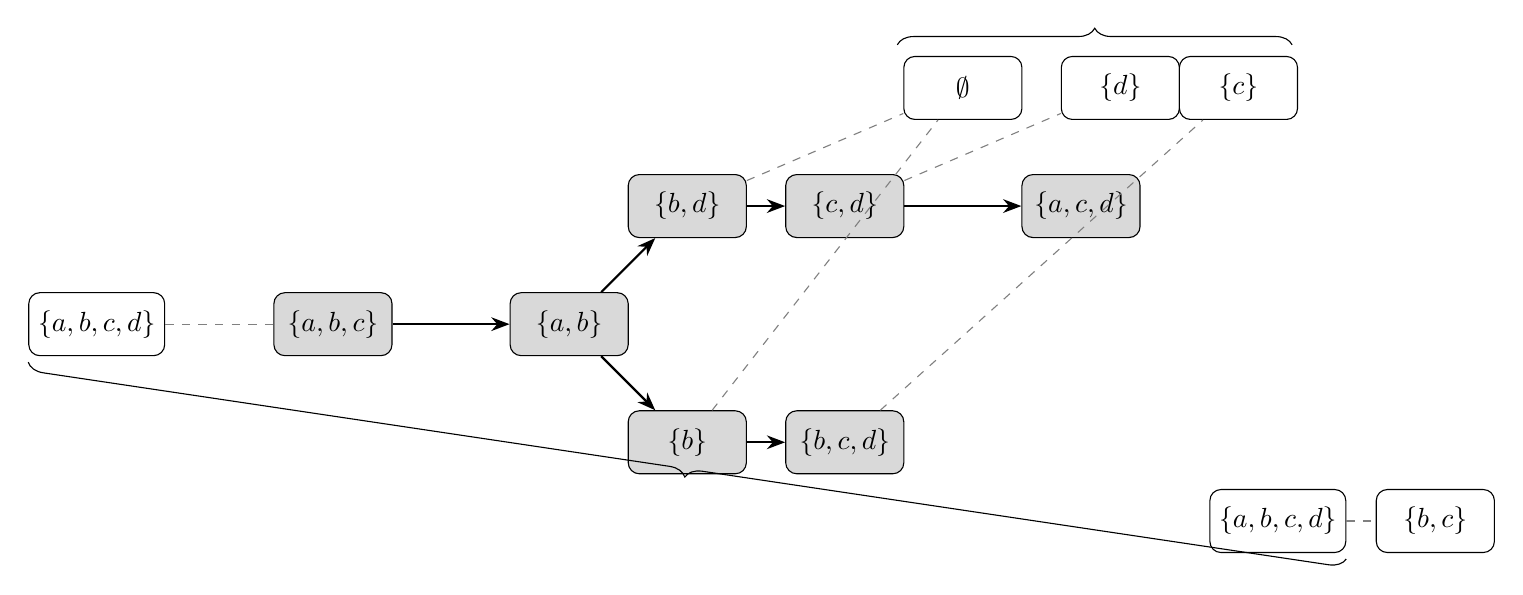
\begin{tikzpicture}[node distance=2cm, >=Stealth]

% Define styles for nodes
\tikzset{
    solution/.style={fill=gray!30, draw=black, rounded corners, minimum width=1.5cm, minimum height=0.8cm},
    regular/.style={draw=black, rounded corners, minimum width=1.5cm, minimum height=0.8cm},
    dashed edge/.style={dashed, gray},
    solid edge/.style={->, thick},
}

% Place nodes
\node[regular] (a_b_c_d) at (0,0) {$\{a,b,c,d\}$};
\node[solution] (a_b_c) at (3,0) {$\{a,b,c\}$};
\node[solution] (a_b) at (6,0) {$\{a,b\}$};
\node[solution] (b_d) at (7.5,1.5) {$\{b,d\}$};
\node[solution] (c_d) at (9.5,1.5) {$\{c,d\}$};
\node[solution] (a_c_d) at (12.5,1.5) {$\{a,c,d\}$};
\node[solution] (b) at (7.5,-1.5) {$\{b\}$};
\node[solution] (b_c_d) at (9.5,-1.5) {$\{b,c,d\}$};
\node[regular] (empty) at (11,3) {$\emptyset$};
\node[regular] (d) at (13,3) {$\{d\}$};
\node[regular] (c) at (14.5,3) {$\{c\}$};
\node[regular] (a_b_c_d_long) at (15,-2.5) {$\{a,b,c,d\}$};
\node[regular] (b_c) at (17,-2.5) {$\{b,c\}$};

% Draw edges
\draw[dashed edge] (a_b_c_d) -- (a_b_c);
\draw[solid edge] (a_b_c) -- (a_b);
\draw[solid edge] (a_b) -- (b_d);
\draw[solid edge] (a_b) -- (b);
\draw[solid edge] (b_d) -- (c_d);
\draw[dashed edge] (b_d) -- (empty);
\draw[dashed edge] (c_d) -- (d);
\draw[solid edge] (c_d) -- (a_c_d);
\draw[solid edge] (b) -- (b_c_d);
\draw[dashed edge] (b) -- (empty);
\draw[dashed edge] (b_c_d) -- (c);
\draw[dashed edge] (a_b_c_d_long) -- (b_c);

% Add braces
\draw[decorate, decoration={brace, amplitude=6pt, mirror}] ([yshift=-0.5ex]a_b_c_d.south west) -- ([yshift=-0.5ex]a_b_c_d_long.south east) node[midway, below, yshift=-1.5em] {};
\draw[decorate, decoration={brace, amplitude=6pt, raise=4pt}] ([xshift=-0.5ex]empty.north west) -- ([xshift=-0.5ex]c.north east) node[midway, above, xshift=1.5em] {};

\end{tikzpicture}
\end{document}